\documentclass[tikz,border=6pt]{standalone}
\usepackage{tikz}
\usepackage{amsmath,amssymb}
\usepackage{xcolor}
\usetikzlibrary{arrows.meta,positioning,calc,decorations.pathmorphing,backgrounds}

% palette
\definecolor{unsafeRed}{HTML}{DC2626}
\definecolor{safeGreen}{HTML}{059669}
\definecolor{promptBlue}{HTML}{2563EB}
\definecolor{winPurple}{HTML}{7C3AED}
\definecolor{unsafeBG}{HTML}{FEE2E2}
\definecolor{safeBG}{HTML}{DCFCE7}
\definecolor{neutralBG}{HTML}{F9FAFB}
\definecolor{greyDark}{HTML}{4B5563}

\begin{document}
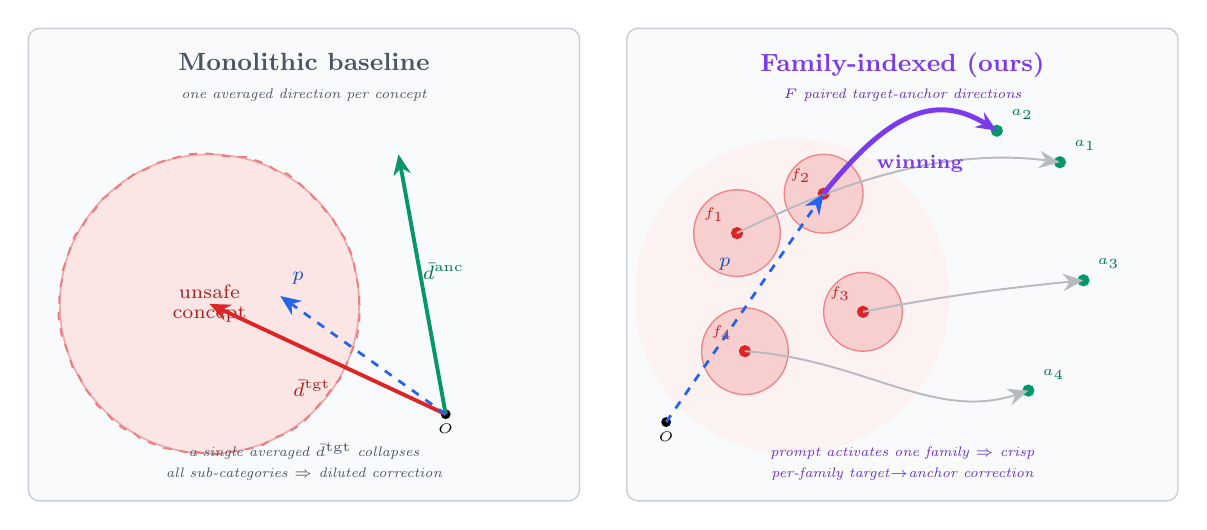
\begin{tikzpicture}[
  font=\footnotesize,
  >={Stealth[length=2.6mm,width=2.2mm]},
  vec/.style={->, line width=1.0pt},
  winvec/.style={->, line width=1.8pt},
  faint/.style={draw=greyDark!30, line width=0.4pt, dashed},
  lbl/.style={font=\scriptsize},
  tinyIt/.style={font=\tiny\itshape},
]

% =============== LEFT : Monolithic baseline ===============
\def\panW{7.0}
\def\panH{6.0}
\def\gap{0.6}

\node[draw=greyDark!30,fill=neutralBG,rounded corners=4pt,line width=0.5pt,
      minimum width=\panW cm,minimum height=\panH cm,anchor=center]
     (panA) at (0,0) {};
\node[anchor=north,font=\small\bfseries,text=greyDark] at ($(panA.north)+(0,-0.20)$)
     {Monolithic baseline};
\node[anchor=north,tinyIt,text=greyDark] at ($(panA.north)+(0,-0.65)$)
     {one averaged direction per concept};

% unsafe region (big blob, soft-fill)
\begin{scope}
\clip[rounded corners=3pt]
  ($(panA.center)+(-\panW/2+0.12,-\panH/2+0.12)$)
  rectangle ($(panA.center)+(\panW/2-0.12,\panH/2-1.30)$);
\fill[unsafeRed!12,draw=unsafeRed!40,line width=0.6pt]
  ($(panA.center)+(-1.2,-0.5)$) circle (1.9);
\draw[unsafeRed!60,line width=0.7pt,dashed,
      decorate,decoration={random steps,segment length=4pt,amplitude=0.6pt}]
  ($(panA.center)+(-1.2,-0.5)$) circle (1.9);
\end{scope}
\node[lbl,anchor=center,text=unsafeRed!80!black]
  at ($(panA.center)+(-1.2,-0.5)$) {\shortstack{unsafe\\concept}};

% origin
\coordinate (OA) at ($(panA.center)+(1.8,-1.9)$);
\filldraw[black] (OA) circle (0.055);
\node[tinyIt,anchor=north] at (OA) {$O$};

% single averaged target (red), toward centroid — label BELOW vector, shifted
\draw[vec,unsafeRed,line width=1.4pt] (OA) -- ($(panA.center)+(-1.2,-0.5)$)
     coordinate (tgtA);
\node[lbl,text=unsafeRed!80!black]
     at ($(OA)!0.45!(tgtA)+(-0.35,-0.30)$) {$\bar d^{\mathrm{tgt}}$};

% single global anchor (green) — points somewhere "safe"
\draw[vec,safeGreen,line width=1.4pt] (OA) -- ($(panA.center)+(1.2,1.4)$)
     coordinate (ancA);
\node[lbl,text=safeGreen!80!black]
     at ($(OA)!0.55!(ancA)+(0.30,0)$) {$\bar d^{\mathrm{anc}}$};

% prompt — label next to tip, well inside unsafe blob area
\draw[vec,promptBlue,dashed,line width=1.0pt] (OA) -- ($(panA.center)+(-0.3,-0.4)$);
\node[lbl,anchor=south west,text=promptBlue!80!black]
     at ($(panA.center)+(-0.27,-0.38)$) {$p$};

% caption under panel
\node[anchor=south,tinyIt,text=greyDark]
     at ($(panA.south)+(0,0.15)$)
     {\shortstack{a single averaged $\bar d^{\mathrm{tgt}}$ collapses\\ all sub-categories $\Rightarrow$ diluted correction}};

% =============== RIGHT : Family-indexed (ours) ===============
\node[draw=greyDark!30,fill=neutralBG,rounded corners=4pt,line width=0.5pt,
      minimum width=\panW cm,minimum height=\panH cm,anchor=center]
     (panB) at (\panW + \gap, 0) {};
\node[anchor=north,font=\small\bfseries,text=winPurple] at ($(panB.north)+(0,-0.20)$)
     {Family-indexed (ours)};
\node[anchor=north,tinyIt,text=winPurple!80!black] at ($(panB.north)+(0,-0.65)$)
     {$F$ paired target-anchor directions};

% unsafe region decomposed into sub-family blobs
\begin{scope}
\clip[rounded corners=3pt]
  ($(panB.center)+(-\panW/2+0.12,-\panH/2+0.12)$)
  rectangle ($(panB.center)+(\panW/2-0.12,\panH/2-1.30)$);
% overall faint outline
\fill[unsafeRed!6] ($(panB.center)+(-1.4,-0.4)$) circle (2.0);
% 4 sub-family blobs
\fill[unsafeRed!22,draw=unsafeRed!55,line width=0.5pt]
  ($(panB.center)+(-2.1,0.4)$) circle (0.55);
\fill[unsafeRed!22,draw=unsafeRed!55,line width=0.5pt]
  ($(panB.center)+(-1.0,0.9)$) circle (0.50);
\fill[unsafeRed!22,draw=unsafeRed!55,line width=0.5pt]
  ($(panB.center)+(-0.5,-0.6)$) circle (0.50);
\fill[unsafeRed!22,draw=unsafeRed!55,line width=0.5pt]
  ($(panB.center)+(-2.0,-1.1)$) circle (0.55);
\end{scope}

% family centroids + labels
\foreach \x/\y/\lab in {-2.1/0.4/f_1, -1.0/0.9/f_2, -0.5/-0.6/f_3, -2.0/-1.1/f_4}{
  \filldraw[unsafeRed]  ($(panB.center)+(\x,\y)$) circle (0.07);
  \node[tinyIt,anchor=south east,text=unsafeRed!90!black]
    at ($(panB.center)+(\x,\y)+(-0.04,0.02)$) {$\lab$};
}

% anchor centroids (safe side — paired same height offset)
\foreach \x/\y/\lab in {2.0/1.3/a_1, 1.2/1.7/a_2, 2.3/-0.2/a_3, 1.6/-1.6/a_4}{
  \filldraw[safeGreen] ($(panB.center)+(\x,\y)$) circle (0.07);
  \node[tinyIt,anchor=south west,text=safeGreen!80!black]
    at ($(panB.center)+(\x,\y)+(0.06,0.02)$) {$\lab$};
}

% paired target->anchor arrows (soft grey) — 3 of them
\draw[vec,greyDark!40,line width=0.7pt]
  ($(panB.center)+(-2.1,0.4)$) .. controls +(1.2,0.6) and +(-1.5,0.2) ..
  ($(panB.center)+(2.0,1.3)$);
\draw[vec,greyDark!40,line width=0.7pt]
  ($(panB.center)+(-0.5,-0.6)$) .. controls +(1.0,0.2) and +(-1.0,-0.1) ..
  ($(panB.center)+(2.3,-0.2)$);
\draw[vec,greyDark!40,line width=0.7pt]
  ($(panB.center)+(-2.0,-1.1)$) .. controls +(1.5,-0.1) and +(-1.2,-0.4) ..
  ($(panB.center)+(1.6,-1.6)$);

% WINNING pair (f_2 -> a_2) highlighted in purple
\draw[winvec,winPurple]
  ($(panB.center)+(-1.0,0.9)$) .. controls +(0.8,1.0) and +(-0.8,0.5) ..
  ($(panB.center)+(1.2,1.7)$);
% The purple arrow itself IS the correction (d^anc_w - d^tgt_w); the exact
% formula is stated in the paper caption, not repeated in-figure.
% One chip marks which family is the winning one for this prompt.
\node[lbl,text=winPurple,anchor=west,font=\scriptsize\bfseries]
  at ($(panB.center)+(-0.45,1.28)$) {winning};

% origin on right
\coordinate (OB) at ($(panB.center)+(-3.0,-2.0)$);
\filldraw[black] (OB) circle (0.055);
\node[tinyIt,anchor=north] at (OB) {$O$};

% prompt direction → routed to winning family (label placed away from f_4 blob)
\draw[vec,promptBlue,dashed,line width=1.0pt] (OB) -- ($(panB.center)+(-1.0,0.9)$);
\node[lbl,anchor=south west,text=promptBlue!80!black]
     at ($(panB.center)+(-2.45,-0.20)$) {$p$};

% caption under panel
\node[anchor=south,tinyIt,text=winPurple!85!black]
     at ($(panB.south)+(0,0.15)$)
     {\shortstack{prompt activates one family $\Rightarrow$ crisp\\per-family target$\to$anchor correction}};

\end{tikzpicture}
\end{document}
